\documentclass[12pt]{article}

\usepackage[utf8]{inputenc}
\usepackage[T1]{fontenc}
\usepackage[spanish]{babel}
\usepackage{graphicx}
\usepackage{listings}
\usepackage{caption}
\usepackage{subcaption}
\usepackage[right=2cm,left=2cm,top=2cm,bottom=2cm]{geometry}
\usepackage{hyperref}
\usepackage{fancyhdr}
\usepackage{color}
\usepackage[export]{adjustbox}
\usepackage{graphicx}
\usepackage{float}
\usepackage{changepage}
\usepackage{multicol}
\usepackage{imakeidx}
\usepackage{csquotes}
\usepackage{array}
\usepackage{tabularx}
\usepackage{xcolor}
\usepackage[backend=biber]{biblatex}

\pagestyle{fancy}
\renewcommand{\footrulewidth}{0.4pt}
\setlength{\headheight}{15pt}


\fancyhead[L]{ CEIABD – PIA }
\fancyhead[R]{ Páez Anguita, Víctor }
\fancyfoot[L]{IES Gran Capitán}


\begin{document}

\begin{titlepage}
    \begin{center}
      \Large \bfseries{}
    \end{center}
    \vspace{0.1cm}
    \begin{center}
      \Large \bfseries{}
    \end{center}
    \vspace{0.1cm}
    \begin{center}
     \Large \bfseries{Data Wrangling con Pandas}
    \end{center}
    \vspace{0.0001cm}
    \begin{center}
        Departamento de informática \\ I.E.S. Gran Capitán - Córdoba
    \end{center}
        \vspace{2 cm}
%\begin{figure}[h!]
%    \centering
%    \includegraphics[width=.6\textwidth]{}
%    \label{fig:my_label}
%\end{figure}
    \vspace{0.2 cm}
    \begin{center}
        Inteligencia artificial y Big data \\ Córdoba, 17 de Noviembre 2024
    \end{center}
    \vspace{12 cm}
\null\hfill \textbf{Desarrollado por:}
\\
\\
\null\hfill Víctor Páez Anguita
\clearpage
\end{titlepage}

%%%%%%%%%%%%%%%%%%%%%%%%%%%Index%%%%%%%%%%%%%%%%%%%%%%%%%%%%%%%%
\tableofcontents
\clearpage
%%%%%%%%%%%%%%%%%%%%%%%%%%%Index%%%%%%%%%%%%%%%%%%%%%%%%%%%%%%%%

\section{Exploración}

La primera vez que abrimos el archivo utilizando la librería de pandas, podemos comprobar que se trata de una lista de clientes
los cuales tenemos distintos datos de cada uno de ellos. La mayoría de estos datos son comunes. Como pueden ser el nombre,
apellidos, dirección, teléfono, etc.
\\
Si profundizamos un poco más en los datos con la función iloc para ver las filas y columnas, veremos que hay datos inncecesarios
o que ya lo obtenemos de una columna. Me refiero al tipo de educación y al oficio del cliente. Que si bien además de poder 
llegar a ser un dato prescindible tenemos esta columna 3 veces en cada una simplemente cambiando la traducción. Para esto
simplemente podríamos obtar por dos opciones:

\begin{itemize}
    \item Eliminar las columnas considerando que no nos interesa ese tipo de información.
    \item Eliminar las columnas y quedarnos con una de ellas.
\end{itemize}

\begin{figure}[h!]
    \centering
    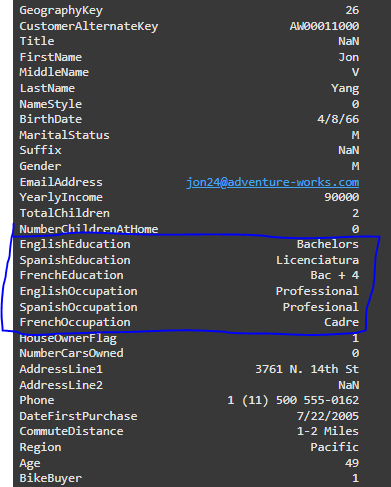
\includegraphics[width=.6\textwidth]{Exploracion1.PNG}
    \label{fig:my_label}
\end{figure}

Siguiendo la exploración de los datos todavía con la función iloc, podemos comprobar que algunos datos de fechas como la de
nacimiento o la de la última compra, tienen distinto formato entre ellos. Algunos el año tiene los 4 dígitos, otros solo 2.
Esto se debe tener en cuenta cuando hagamos una limpieza de los datos.
\\
Continuando con más datos que podemos descartar tenemos la segunda dirección que practicamente esta vacía en todos los clientes.
El "Suffix" el cual es una columna vacía y que no aporta ningún tipo de información, al igual que el NameStyle.
Por último el campo "title", el cual es un campo al igual que el anterior vacío e irrelevante.

\begin{figure}[h!]
    \centering
    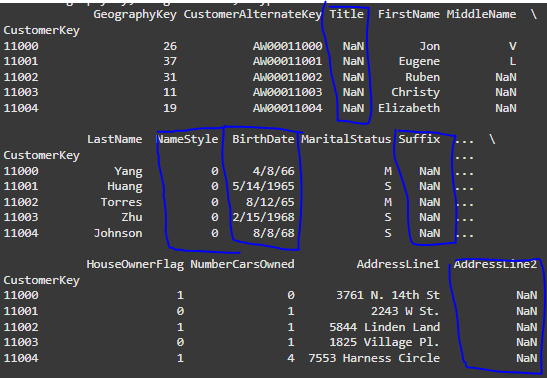
\includegraphics[width=.6\textwidth]{Exploracion2.PNG}
    \label{fig:my_label}
\end{figure}

Continuando con la exploración del archivo, si sacamos un data.info() podemos observar que la mayoría de los datos son 
objetos, a tener en cuenta en la limpieza de los datos. Si seguimos con este tipo de dato o cambiarlo.
\\
Siguiendo si sacamos para ver cuantos valores distintos hay por cada columna observamos que hay una gran variedad por lo que
nuestro dataset es bastante completo.
\\
Por último si comprobamos los valores nulos exceptuando aquellos campos comentados anteriormente, podemos ver como no hay 
ningún valor nulo, por lo que facilitará las proxiamas tareas sobre este.
\\
Desde este enlace al colab, se puede ver la exploración de los datos de una manera más visual y siguiendo todo el proceso que
hemos hecho para llegar a estas conclusiones.

\begin{itemize}
    \item \href{https://colab.research.google.com/drive/1pA3PSNv5cui1JHyDh54nvRc1NihJn-0F?usp=sharing}{Colab}
\end{itemize}


\end{document}
